% Chapter Template

\chapter{Literature Review} % Main chapter title
%\doublespacing
\label{Chapter2} % Change X to a consecutive number; for referencing this chapter elsewhere, use \ref{ChapterX}
\section{Molecular Simulations of Molecules Mimicking Asphaltenes}
Asphaltenes consist of polyfunctional molecules, and they are defined by their solubility: insoluble in n-alkanes (pentane, hexane and heptane) and solube in tolune. Due to uncertainties related to its structures, a lot work has been done to develop model compounds that have well defined structure and can represent an average asphaltene. The two category of models presented in the literature are the archipelago and continental models. In the archipelago, asphaltenes consist of polyaromatic parts linked together by aliphatic or naphthemic moieties and, in the continental, they consist of a single
polyaromatic ring with linked aliphatic or naphthenic chains \cite{doi:10.1021/ef900975e,doi:10.1080/0892702031000148762}. Studies with molecular simulation uses this models or compounds, such as like toluene and pyrene, that have similar solubility properties. The model's structure as chemical bonding  can cause high energies during the simulation and, consequently, low relative occurrence probabilities \cite{doi:10.1021/ef200507c} .   

\citeonline{ERVIK2016576}  obtained correct interfacial orientation of asphaltenes using coarse grained molecular dynamics simulations of the interface, with an accurate model for the asphaltene molecules. Using a coarse grained force field also, \citeonline{doi:10.1021/ef502209j} carried molecular simulations with a continental asphaltene model. The results reproduced experimental data if the strong aggregation
of asphaltene molecules in n-heptane and high solubility in toluene. Meanwhile, \citeonline{doi:10.1021/ef5020428} performed a molecular
dynamics study with the force field GROMOS 45a3 force field to identify the structural features of different asphaltene molecules (C5 Pe and
anionic C5 Pe). The archipelago model was employed in the work of \citeonline{doi:10.1021/ef301610q} to investigate interfacial behavior of asphaltene molecules at the oil - water interface using molecular dynamics simulations with the OPLS-AA force field. They found that  asphaltenes are preferably distributed in the oil phase in the case of pure toluene and at the oil - water interface
in the case of pure heptane. A molecular
oscillation behavior of asphaltene molecules at the oil - water interface was also discovered in the shape of a nanoscale aggregate.

A pyrelene based model was used in the work of \citeonline{doi:10.1021/jp3010184,doi:10.1021/jp407363p} to study molecular association and interaction as well as the adsorption properties of the pyrelene model at the water/toluene or heptane interface. Molecular dynamics simulations were also used to the study the nanoaggregation of four types of model asphaltene molecules in binary mixtures of toluene and water \cite{doi:10.1021/ef9004576}. This study observed that  in thin films of toluene trapped between two aqueous phases,
both interface-bound and core-bound asphaltenes have similar diffusion behavior. \citeonline{doi:10.1021/acs.energyfuels.6b02161} reported molecular dynamics simulations of four model asphaltenes. They aver that there is no formation of nanoaggregates, and the distribution of clusters is continuous for mixtures of asphaltene in heptane. Generally the works on molecular simulation with asphaltenes models showed a difference in
packing tendencies according to the model \cite{doi:10.1080/10298436.2011.575141}. For a thorough review of studies of different models of asphaltenes, the reader is referred elsewhere \cite{doi:10.1080/10298436.2011.575141}. 


\section{Coarse Grained Force Fields}


Molecular simulations can be carried out at different levels of description. The detailed atomistic level or \textit{ab initio} level is described by the laws of quantum mechanics. The system consists of a set of subatomic particles in which Schrodinger's equation is solved for all of them. The next level is the atomistic description. It considers that the system is made up of atoms following the laws of statistical mechanics.  Force fields at this level are based on pair potentials with Coulombic charged sites. Contributions due to intramolecular interactions such as bond-stretching, angle-bending and torsion are also usually accounted by these kinds of force fields. When the simulation scale needs to be increased and the atomistic simulations become too computationally expensive, the coarse-grained (CG) description is more suited. It considers that the system is made up of pseudo atoms or beads that contain multiple atoms or even an entire molecule. 

There is an obvious loss of information in grouping atoms, hence it is necessary to assure that the process of eliminating unnecessary or unimportant information ('coarse graining') doesn't affect the system's physical behavior. Ideally, coarse grained models need to have accuracy, transferability, robustness, and computational efficiency. In order to achieve these goals, coarse grained force fields are usually developed by mapping the atomistic model in order to define the pseudo atoms, which are generally formed by similar functional groups. The level of coarse graining also needs to be defined, up to 6 heavy atoms (non-hydrogen atoms) per bead in order to not lose important details and maintain isotropic representations of the beads \cite{shinoda2007,martini2007,hadley2012}. CG force fields can be parametrized following two different approaches, bottoms up and top down, to link the simulations on the coarse grained scale to a more detailed scale according to the schematic representation in \figref{fig:multiscale}. The bottoms up approach uses information of a more detailed scale such as the \textit{ab initio} description or the atomistic description to obtain information necessary to the parametrization. This method highly depends on the detailed model quality to succeed. Meanwhile, the top down methodology obtains parameters from larger scales, namely experimental thermodynamic properties or native-structure based properties. 

\begin{figure}{H}
	\centering
	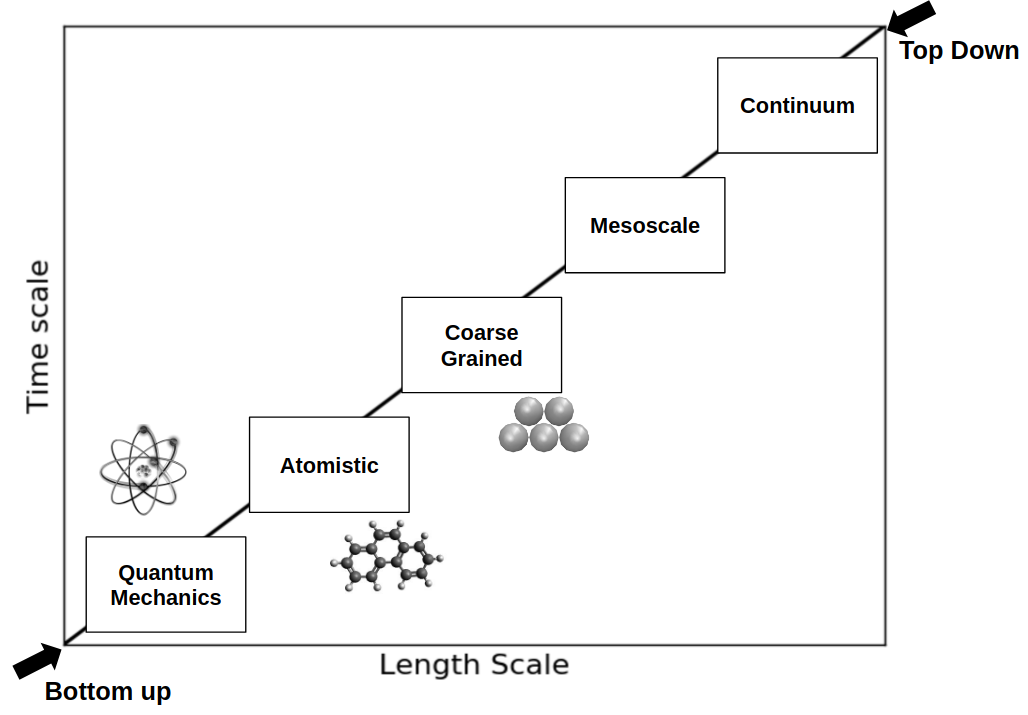
\includegraphics[width=0.8\linewidth]{Figures/multiscale}
	\caption{Schematic representation for the two different approaches of coarse graining.Taken from \citeonline{tatyana}}
	\label{fig:multiscale}
\end{figure}
\FloatBarrier

One of the first applications of coarse grained models is the study of protein folding \cite{levitt1975,levitt1976}. These earlier protein CG models were based on molecule structure, and they contributed for the knowledge of physicochemical forces associated with protein folding and protein interactions \cite{koga2001}.  More recent, models focused on retaining the protein's chemical specificity. The Bereau and Deresmo model \cite{bereau2009} has up to four-bead representation and was used in studies of protein folding and aggregation. However, this model still needs tuning to improve protein stability \cite{bereau2010}. The OPEP (Optimized Potential for Efficient Protein Structure Prediction) model \cite{opep2014,opep2015} has up to six-bead representation. It was used to investigate a variety of phenomenon, ranging from protein folding to \textit{ab initio} peptide structure prediction \cite{opep2011,opep2009,opep20092}. Another CG protein models used in the literature are the Scorpion (solvated coarse-grained protein interaction)  \cite{scorpion2013}, the UNRES (united residue) \cite{unres2014} and the MARTINI model \cite{martini2013}. The later one is the most popular model for CG modeling of membrane proteins \cite{martini20132}. The MARTINI model is also extensively used as CG model for water. This model represents four water molecules as one bead using a shifted Lennard Jones potential for non bonded interactions. Though its extensive use, the MARTINI water model doesn't properly represent properties as interfacial tension and compressibility \cite{shinoda2010} and can freeze at room temperature \cite{winger2009,martini2007}, what requires the use of anti-freeze agents during the simulations. This behavior can be explained by the high level of coarse graining (4:1), the lack of explicit charges and the use of a 12-6 potential. \citeonline{chiu2010} used the Morse Potential, which is softer than the LJ potential, to improve the MARTINI model. Meanwhile, \citeonline{shinoda2007} used different forms of the Mie potential. They concluded that a 12-4 Mie Potential was ideal for water cross interactions and  a 9-6 Mie Potential was suited for solute-solute interactions. 

Outside of the Martini framework, \citeonline{shinoda2010} studied different levels of coarse-graining for water ranging for one to 4 molecules per bead using different Mie and Morse potentials. Works also assessed the use of Soft-core potentials to study aqueous solutions of surfactants \cite{shinoda2007}, ionic liquids \cite{bhargava2009}, lipids \cite{shinoda20102} and membranes \cite{pantano2009}. Another CG force field for water based on the Mie Potential is the SAFT-$\gamma$ Mie \cite{lobanova2015}. In this strategy, there are two different models: the CGW1-vle and the CGW1-ift. Both of them represent the water molecule as one bead and  the Mie Potential has a repulsive and attractive parameter equal to eight and six, respectively. The CGW1-vle model was parameterized using saturated-liquid density and vapor pressure data, and should be used for simulations of aqueous systems' fluid-phase equilibrium at high temperatures and pressures. This model still suffers from premature freezing with a triple point at 343 K. The other model, CGW1-ift, was parameterized using saturated-liquid density and vapor-liquid interfacial tension, hence it is best suited for interfacial properties calculations. Both models have temperature-dependent size and energy parameters and performed well for these properties over the entire liquid temperature range. The SAFT-$\gamma$ Mie force field have also been applied to other compounds with satisfactory results. \citeonline{muller2017} parameterized the force field for aromatic compounds and tested it with simulations of fluid phase equilibrium. \citeonline{herdes2015} carried out simulations of alkanes and light gases. Binary and ternary mixtures of water, carbon-dioxide and water \cite{lobanova2016}, thermodynamic and transport properties of carbon dioxide and methane \cite{cassiano1,cassiano2} and water/oil interfacial tension \cite{herdes2017} were also studied with this force field.  



%----------------------------------------------------------------------------------------
%	SECTION 2
%----------------------------------------------------------------------------------------
\section{Solvation Free Energies}

Solvation free energy calculations with molecular dynamics have a variety of applications due the amount of information it can provide about the behavior of the solvent in different chemical environments and the influence of the solute's molecular geometry. Free energy calculations have an inherent complexity that attracted studies in order to  improve free energy simulations and post processing methods \cite{mbar,bareva,dexp,gdel} in the last decades.

Recent work \cite{PMID:24928188,mobley2017} made available a big database of hydration free energy of small molecules using the GAFF force field. \citeonline{Beckstein2014} also calculated the hydration free energies for 52 compounds with OPLS-AA force field. They obtained an overall root mean square deviation of the prediction from the experimental data of 1.75 kcal/mol and concluded that the precision of the results are mainly limited by the reproducibility of the Lennard-Jones contribution towards the solvation free energy. A comparison of polar and nonpolar contributions to these hydration free energy indicated the significance of each the terms  \cite{izairi2017}. \citeonline{garrido,garrido2011} calculated the free energy of solvation of large alkanes in 1-octanol and water with three different force fields (TraPPE, Gromos, OPLS-AA/TraPPE) and the solvation free energy of propane and benzene in non aqueous solvents like n-hexadecane, n-hexane, ethyl benzene and acetone  with the force fields TraPPE-UA and TraPPE-AA. \citeonline{roy2017} addressed the choice of the Lennard Jones parameters for predicting solvation free energy in 1-octanol. \citeonline{goncalves} calculated the free energy of solvation in the solvents tetrachloride, chloroform and benzene with GROMOS force field. Using the GAFF and the polarizable AMOEBA force fields, \citeonline{mohamed2016} evaluated the solvation free energy of small molecules in toluene, chloroform and acetonitrile, and obtained a mean unsigned error of 1.22 kcal/mol for AMOEBA and 0.66 kcal/mol for GAFF. In order to define the role of solvent water in the docking structure determination, \citeonline{MATUBAYASI201745} developped a method to compute the solvation free energy of proteins while using OPLS-AA force field for the
solutes and TIP3P for water. \cite{doi:10.1021/acs.jctc.5b00963} used a coarse grained model created with the Elba force field to calculate solvation free energies in polar (water, hexanol, octanol and nonanol) and apolar (hexane,octane and nonane) solvents, and obtained mean absolute deviations of 1 kcl/mol for water and 1.5 kcal/mol for hexane. In this model, three carbons are represented by a single bead and water is represented by a single bead. 

Though these variety of data using the intramolecular Lennard-Jones potential, we are not aware of works using the Mie Potential\cite{MIE} in free energy calculations. We, at this study, try to provide information about theses calculations with the SAFT-$\gamma$ Mie coarse grained force field.  The output of these calculations are highly dependent on the force field and deficiencies in the description of small molecules by the models can be revealed with these calculations \cite{mobley2007,shirts2013}. Other important reason for testing a coarse grained force field is that they can generally reproduce free energy difference since the effects of the degrees of freedom reduction  in the entropy are counterbalanced by reduced enthalpic terms \cite{kmiecik2016}. Hence, knowing if more coarse grained approaches have a similar performance to the all atoms force fields can help increase the scale of solvation free energy calculations. 

\section{Solvation Free Energies Calculation Methods}

The data from molecular dynamics simulations provide potential energies that need to be post processed and analyzed in order to calculate the solvation free energies. Since these calculations  can have slow convergences, a lot of papers in the last decades focused in developing methods to improve sampling and analysis techniques. Almost all methods rely o three different approaches: free energy of perturbation (FEP), histogram and thermodynamic integration methods.

\subsection{Thermodynamic integration}

The thermodynamic integration method \cite{kirkwood1935} uses equilibrium averages to evaluate the energy derivative with respect to the coupling parameter ($\lambda$): 
%Then, the free energies are calculated by  doing the derivative ($\frac{\partial G}{\partial \lambda} $):
%
%\begin{equation}
%\label{eq:ti1}
%\begin{aligned}
%\frac{\partial \beta G}{\partial \lambda} = - \frac{1}{Z (\lambda)}\frac{\partial Z}{\partial \lambda}
%\end{aligned}
%\end{equation}
%
%The Eq. \eqref{eq:dif} can be rewritten according to the Halmitonian of the system ($\mathcal{H}$):
%
%\begin{equation}
%\label{eq:ti2}
%\begin{aligned}
%\Delta G = - \kappa_{b}T ln \left( \frac{Z_{1}}{Z_{0}}\right) = -\kappa_{b}T ln \int \frac{exp(-\beta \mathcal{H} _{1}(r,p)) dr dp}{exp(-\beta \mathcal{H} _{0}(r,p)) dr dp}
%\end{aligned}
%\end{equation}

%Substituting Eq. \eqref{eq:ti2} in \eqref{eq:ti2} and adding the coupling parameter to the Halmitonian ($\mathcal{H} (r,p,\lambda)$) in order to describe the transition between the end states:

%\begin{equation}
%\label{eq:ti3}
%\begin{aligned}
%\frac{\partial \beta G}{\partial \lambda} =  \int \frac{\frac{\partial \mathcal{H} (r,p,\lambda)}{\partial \lambda}exp(-\beta \mathcal{H}(r,p,\lambda)) dr dp}{exp(-\beta \mathcal{H}(r,p,\lambda)) dr dp} =  \left \langle \frac{\partial \mathcal{H}(r,p,\lambda)}{\partial \lambda} \right \rangle 
%\end{aligned}
%\end{equation}

\begin{equation}
\label{eq:ti3}
\begin{aligned}
\frac{\partial (1/k_{b}T) G}{\partial \lambda} =  \left \langle \frac{\partial \mathcal{H}}{\partial \lambda} \right \rangle 
\end{aligned}
\end{equation}

In Eq. \eqref{eq:ti3}, $k_{b}$ is the Boltzmann constant, $G$ is the Gibbs free energy and $\mathcal{H}$ is the Halmitonian of the system. The derivative is obtained by interpolating the output data between the states from simulations. Some examples of methods for the interpolations are the trapezoidal rule or natural cubic spline \cite{bareva}. There are also more complex schemes that are usually system specific as the works of \citeonline{garrido2010} and \citeonline{shyu2009}. MD simulations for each coupling parameter $k$ are carried out and the average over the derivative at each state is compute in order to obtain the final solvation free energy:

\begin{equation}
\label{eq:ti4}
\begin{aligned}
\Delta G \approx \sum _{k}  \left \langle \frac{\partial \mathcal{H}}{\partial \lambda} \right \rangle 
\end{aligned}
\end{equation}

\subsection{Histograms}
%97
Histograms are used  to compute probability distributions. Usually every histogram bin is treated as number of visits to a specific state.The standard practice when using histograms is to use the weighted histogram analysis method (WHAM) developed by \citeonline{PhysRevLett.63.1195} and generalized by \citeonline{wham} \cite{freeenergy} to put together different histograms by minimizing the statistical error in the computed density of states and entropy function. This method describes the total probability distribution as a weighted sum of probability distributions without bias  obtained from biased simulations. This method was developed to avoid problems related to data loss, high uncertainties and the calculation of the constant of the free energy added to the system by the biased potential \cite{ROUX1995275}. The probability distribution dependent on the potential energy ($U$) and temperature (T) ($\tilde{\varrho_{r}^{*}}(U,T)$) for the WHAM is:

\begin{equation}
\label{eq:wham1}
\tilde{\varrho_{r}^{*}}(U,T) = \frac{\sum_{i} f_{i}(U) exp(- \beta U)}{\sum_{i} f_{tot,i} exp(\beta _{i} \tilde{A}_{i} -\beta _{i} U) }
\end{equation} 

\begin{equation}
\label{eq:wham2}
exp(- \beta _{i} \tilde{A}_{i}) = \sum_{U} \tilde{\varrho_{r}^{*}}(U,T) 
\end{equation}

\begin{equation}
\label{eq:wham3}
\tilde{\varrho_{r}^{*}}(U,T) = \frac{\tilde{\varrho_{r}^{*}}(U,T)}{\sum_{U} \tilde{\varrho_{r}^{*}}(U,T)}
\end{equation} 
where $\beta = 1/k_{b}T$, $\tilde{A}_{i}$ gives the free energy for run i, $f_{i}(U)$ is the number of counts of energy U for run i and $f_{tot,i}$ is the total number of counts in run i. The Eq. \eqref{eq:wham1} and \eqref{eq:wham2} are solved self consistently with the initial value for $\tilde{A}_{i}$ equal to zero. The final probability distribution is then given by Eq. \eqref{eq:wham3}, and is used to calculate various moments of the potential energy \cite{freeenergy}.


\subsection{Free Energy of Perturbation (FEP)}
%38
The free energy of perturbation method \cite{zwanzig1954} is the oldest and one of the most general purpose strategy to calculate free energy differences. In this method, the thermodynamics of two different systems( A and B) are related with the intention of evaluating differences in intermolecular potentials. This energy change from state A to state B is calculated by:  

\begin{equation}
\label{eq:fep}
\begin{aligned}
\Delta G_{AB} = -k_{b}T ln \langle{e^{-\beta (U_{B}-U_{A})}}\rangle_{A}
\end{aligned}
\end{equation}

According to the equation above, the free energy difference is calculated by doing an average over the potential energies of state A and B obtained during the simulation of state A. This method requires a great overlap between states( the state B needs to represent a small perturbation in state A) in order to obtain a rapid convergence of the free energy difference. To assure overlap, it is possible to carry out simulations in N intermediate states between A and B, so Eq. \eqref{eq:fep} becomes:

\begin{equation}
\label{eq:fepint}
\begin{aligned}
\Delta G_{AB} = -k_{b}T  ln \left(\frac{1}{N}\sum_{i=0}^{N+1}
{e^{-\beta (U_{i+1}-U_{i})}}\right)_{i}
\end{aligned}
\end{equation}

The way of calculating $\Delta G$ of Eq. \eqref{eq:fepint} is called Exponential Averaging (EXP) \cite{zwanzig1955,bareva}. The direction of the transformation is also important in this method. If the direction is of decreasing entropy, the step is of insertion ($\Delta G_{AB}$) and the method is called insertion exponential averaging (IEXP). The direction of increasing entropy is  called a deletion step ($\Delta G_{BA}$) and the method is labeled as deletion exponential averaging (DEXP). These directions can yield different values of free energy differences due to under sampling in the tail regions of the $\Delta G_{AB}$ distribution \cite{klimovich,pohorille2010}. These problems make the EXP methods not suited to calculate free energy differences when the system hasn't a sufficient overlap. For these cases, the Bennet Acceptance Ratio or the Multi-State Bennet Acceptance Ratio is more indicated.   

\subsubsection{Bennet Acceptance Ratio (BAR)}

The BAR method \cite{bennet1976} was developed with the intent of eliminating the bias in the free energy estimation. It uses the uncorrelated samples of the potential energy in both directions ($A \rightarrow B$ and $B \rightarrow A$) to obtain the free energy differences using the information in a statically optimal way. The free energy difference between two intermediate states (i and j) is calculated by the self-consistent solution of the following equations: 

\begin{equation}
\label{eq:bar1}
\begin{aligned}
\Delta G_{ij} = \frac{1}{\beta} ln \left( \dfrac{\sum_{k=1}^{N_{j}} \dfrac{1}{1+\exp[-\beta(\Delta U_{k}^{j}-C)]}}{\sum_{l=1}^{N_{i}} \dfrac{1}{1+\exp[-\beta(\Delta U_{l}^{i}-C)]}}\right) + C - \frac{1}{\beta}ln\left(\frac{N_{j}}{N_{i}}\right)
\end{aligned}
\end{equation}

\begin{equation}
\label{eq:bar2}
\begin{aligned}
C = \Delta G_{ij} + \frac{1}{\beta}ln\left(\frac{N_{j}}{N_{i}}\right)
\end{aligned}
\end{equation}

The total free energy difference between end states is then given by the sum over differences of consecutive intermediate states. This method also provides a function to obtain the minimum variance for free energy differences. The variance equation for any value of C is given by:

\begin{equation}
\label{eq:barvar}
\begin{aligned}
s_{ij}^{2} = \frac{1}{\beta^{2} N_{i}} \left[\dfrac{\langle{f^{2}(x)}\rangle_{i}}{\langle{f(x)}\rangle^{2}_{i}} - 1\right] + \frac{1}{\beta^{2} N_{j}} \left[\dfrac{\langle{f^{2}(x)}\rangle_{j}}{\langle{f(x)}\rangle^{2}_{j}} - 1\right]
\end{aligned}
\end{equation}
where $f(x)=1/(1+x)$ is the Fermi equation and $x=\exp[\beta(\Delta U - C)]$. The variance of the free energy difference between end states can be calculated by assuming independent errors and summing over the variance of consecutive intermediate states. However, this assumption is not correct and there is no general formula to obtain a statistically unbiased estimate of an entire transformation with the BAR method \cite{bareva}. 

There are two other methods related to the BAR method that don't solve Eqs. \eqref{eq:bar1} and \eqref{eq:bar2} self consistently. By doing that, free energy differences will not have minimum variance, but significant space and disk memory can be saved since the averages of Eqs. \eqref{eq:bar1} - \eqref{eq:barvar} are accumulated\cite{bareva}. The two methods are the Unoptimized Bennett Acceptance Ratio (UBAR) and the Range-Based Bennett Acceptance Ratio (RBAR). The first one avoids the self consistently resolution of the BAR equations by defining $C=\beta^{-1}ln(N_{j}/N_{i})$. The UBAR method also requires that the intermediate free energy differences are approximately equal to zero to obtain optimal estimations. Meanwhile, the RBAR method selects a range of initial guesses of the constant $C$ in order to calculate a range  of $\Delta G_{ij}$. The value of free energy difference correspondent to the minimum variance is then used as input in Eq. \eqref{eq:bar2} to calculate the value of $C$. Hence, this method requires a good estimation of the initial range for the values of $C$. In terms of accuracy, the UBAR method can be as accurate as the BAR method, but it may end up being as computational costly \cite{bareva}.  

\subsubsection{Multistate Bennet Acceptance Ratio (MBAR)}

The MBAR method \cite{mbar} is a further development of the BAR method. It proposes an estimator that computes free energies and their uncertainties of all $K$ states  by minimizing the $KxK$ matrix of variances simultaneously. The estimator solves the following equation for each $G_{i}$ self consistently:

\begin{equation}
\label{eq:mbar}
\begin{aligned}
G_{i} = \frac{1}{\beta}ln \sum_{k=1}^{K} \sum_{n=1}^{N_{k}}
\dfrac{\exp[-\beta U_{i}(x_{kn})]}{\sum_{l=1}^{K} N_{l} \exp[\beta (G_{l} - U_{l}(x_{kn}))]}
\end{aligned}
\end{equation}

The equation above requires the evaluation of the potential energy  of uncorrelated configuration $n$ for all K states ($U_{i}(x_{kn}$) and for all uncorrelated configuration snapshots ($N_{k}$) from state $k$. Free energy changes between states are given then by $\Delta G_{ij} = G_{j} -  G_{i}$. The statistical variance of $S_{ij}^{2} \Delta G_{ij}$ is given by the matrix covariances:

\begin{equation}
\label{eq:varmbar}
\begin{aligned}
s_{ij}^{2} \Delta G_{ij} \equiv cov (-ln \hat{Z_{j}}/\hat{Z_{i}},-ln \hat{Z_{j}}/\hat{Z_{i}})
\end{aligned}
\end{equation}
where $\hat{Z_{j}}$ and $\hat{Z_{i}}$ are the partition functions of states $i$ and $j$. 
